\subsection{A Quick Overview of Parallel Hardware}
\makesubcontentsslidessec

\begin{frame}{Three Basic Flavors of Hardware}
\includegraphics[width=0.95\textwidth]%
{../common/pics/hardware/ParallelHardware1.pdf}
\end{frame}

\begin{frame}{Your Laptop or Desktop}
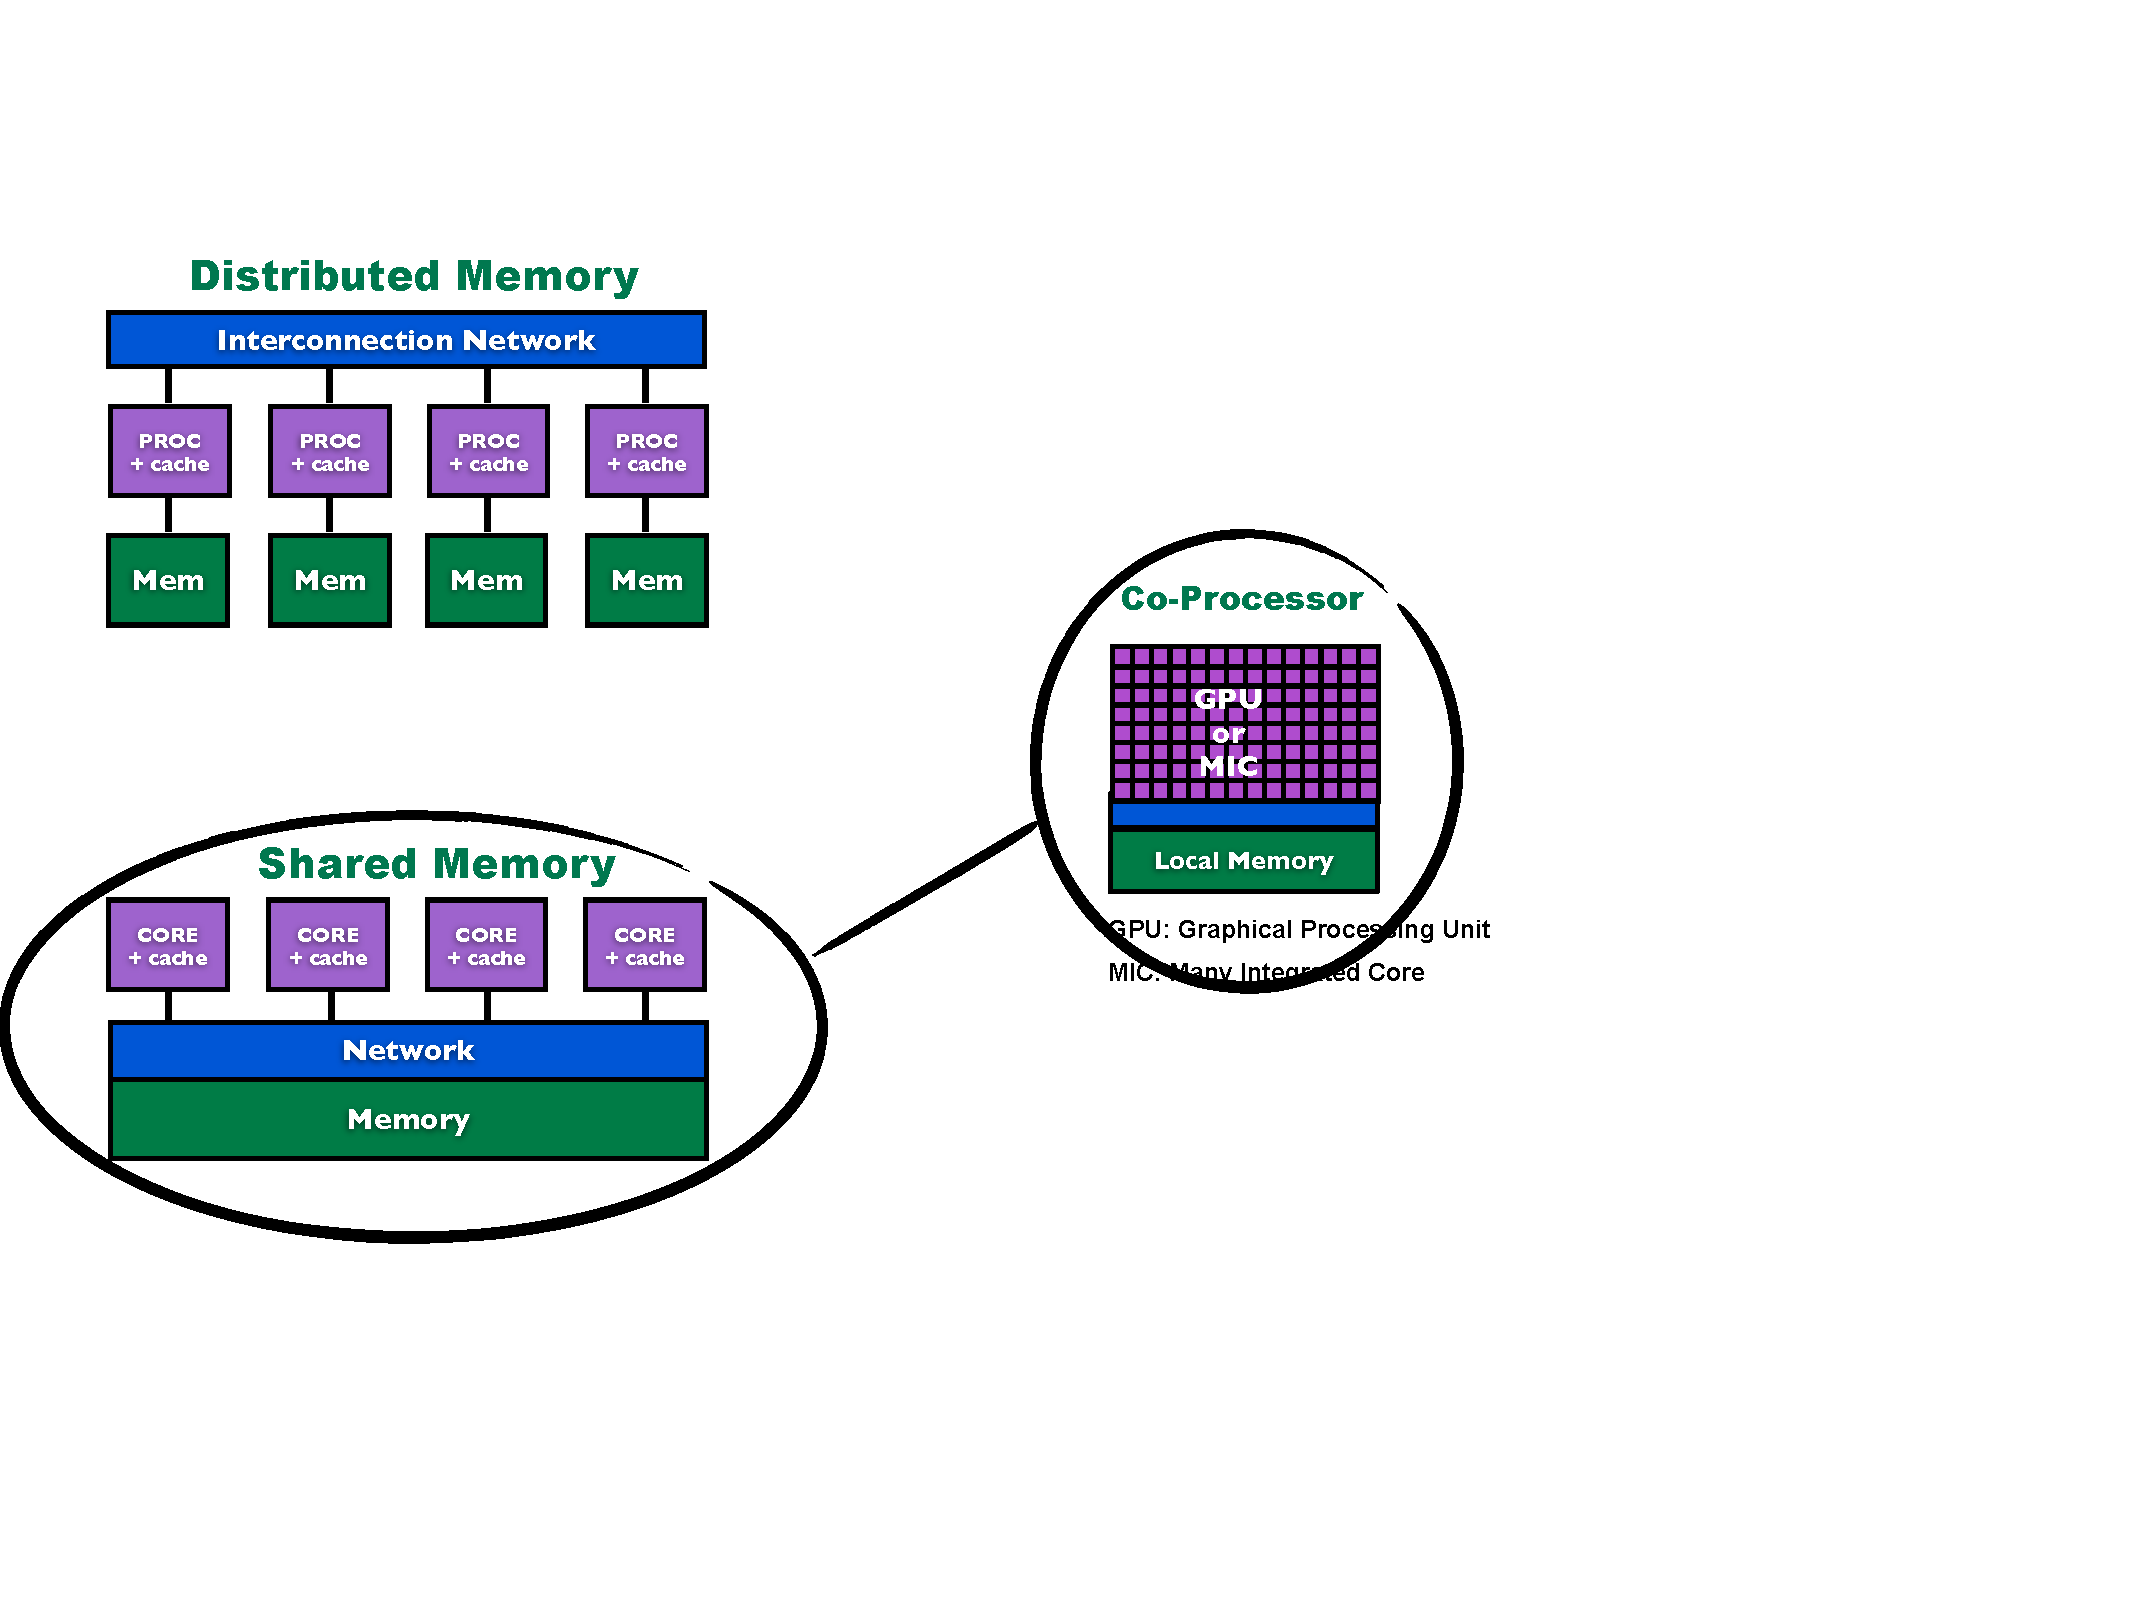
\includegraphics[width=0.95\textwidth]
{../common/pics/hardware/ParallelHardware2.pdf}
\end{frame}

\begin{frame}{A Server or Cluster}
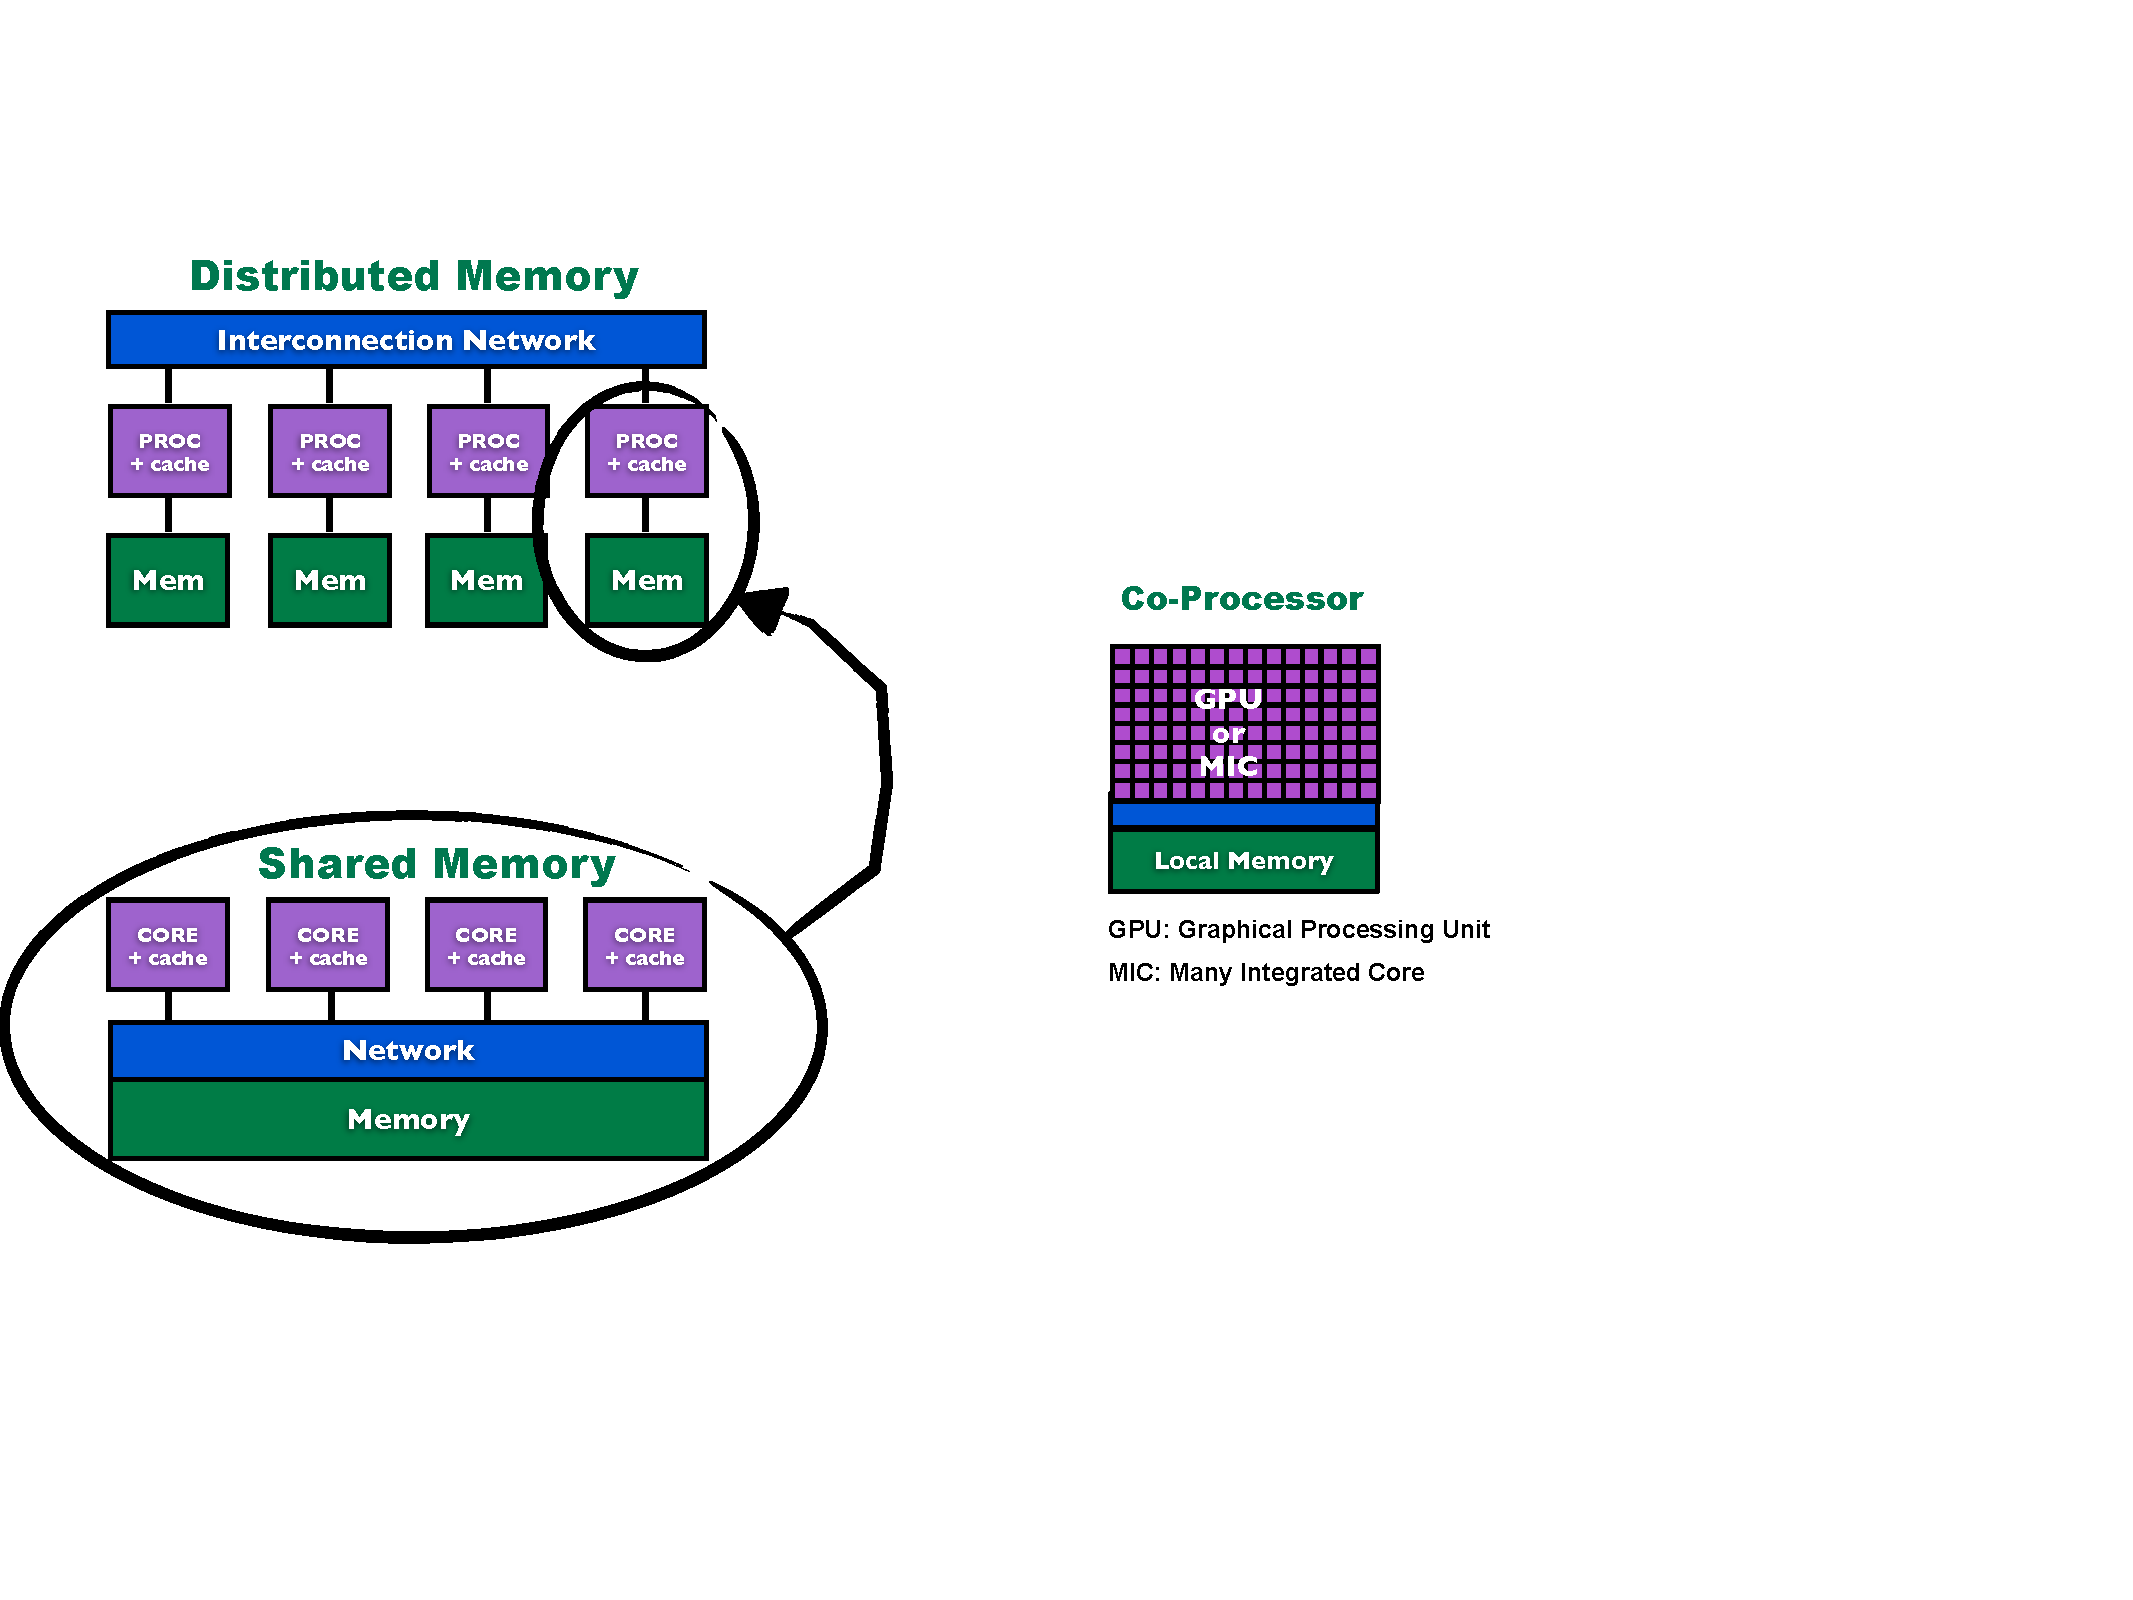
\includegraphics[width=0.95\textwidth]
{../common/pics/hardware/ParallelHardware3.pdf}
\end{frame}

\begin{frame}{Server to Supercomputer}
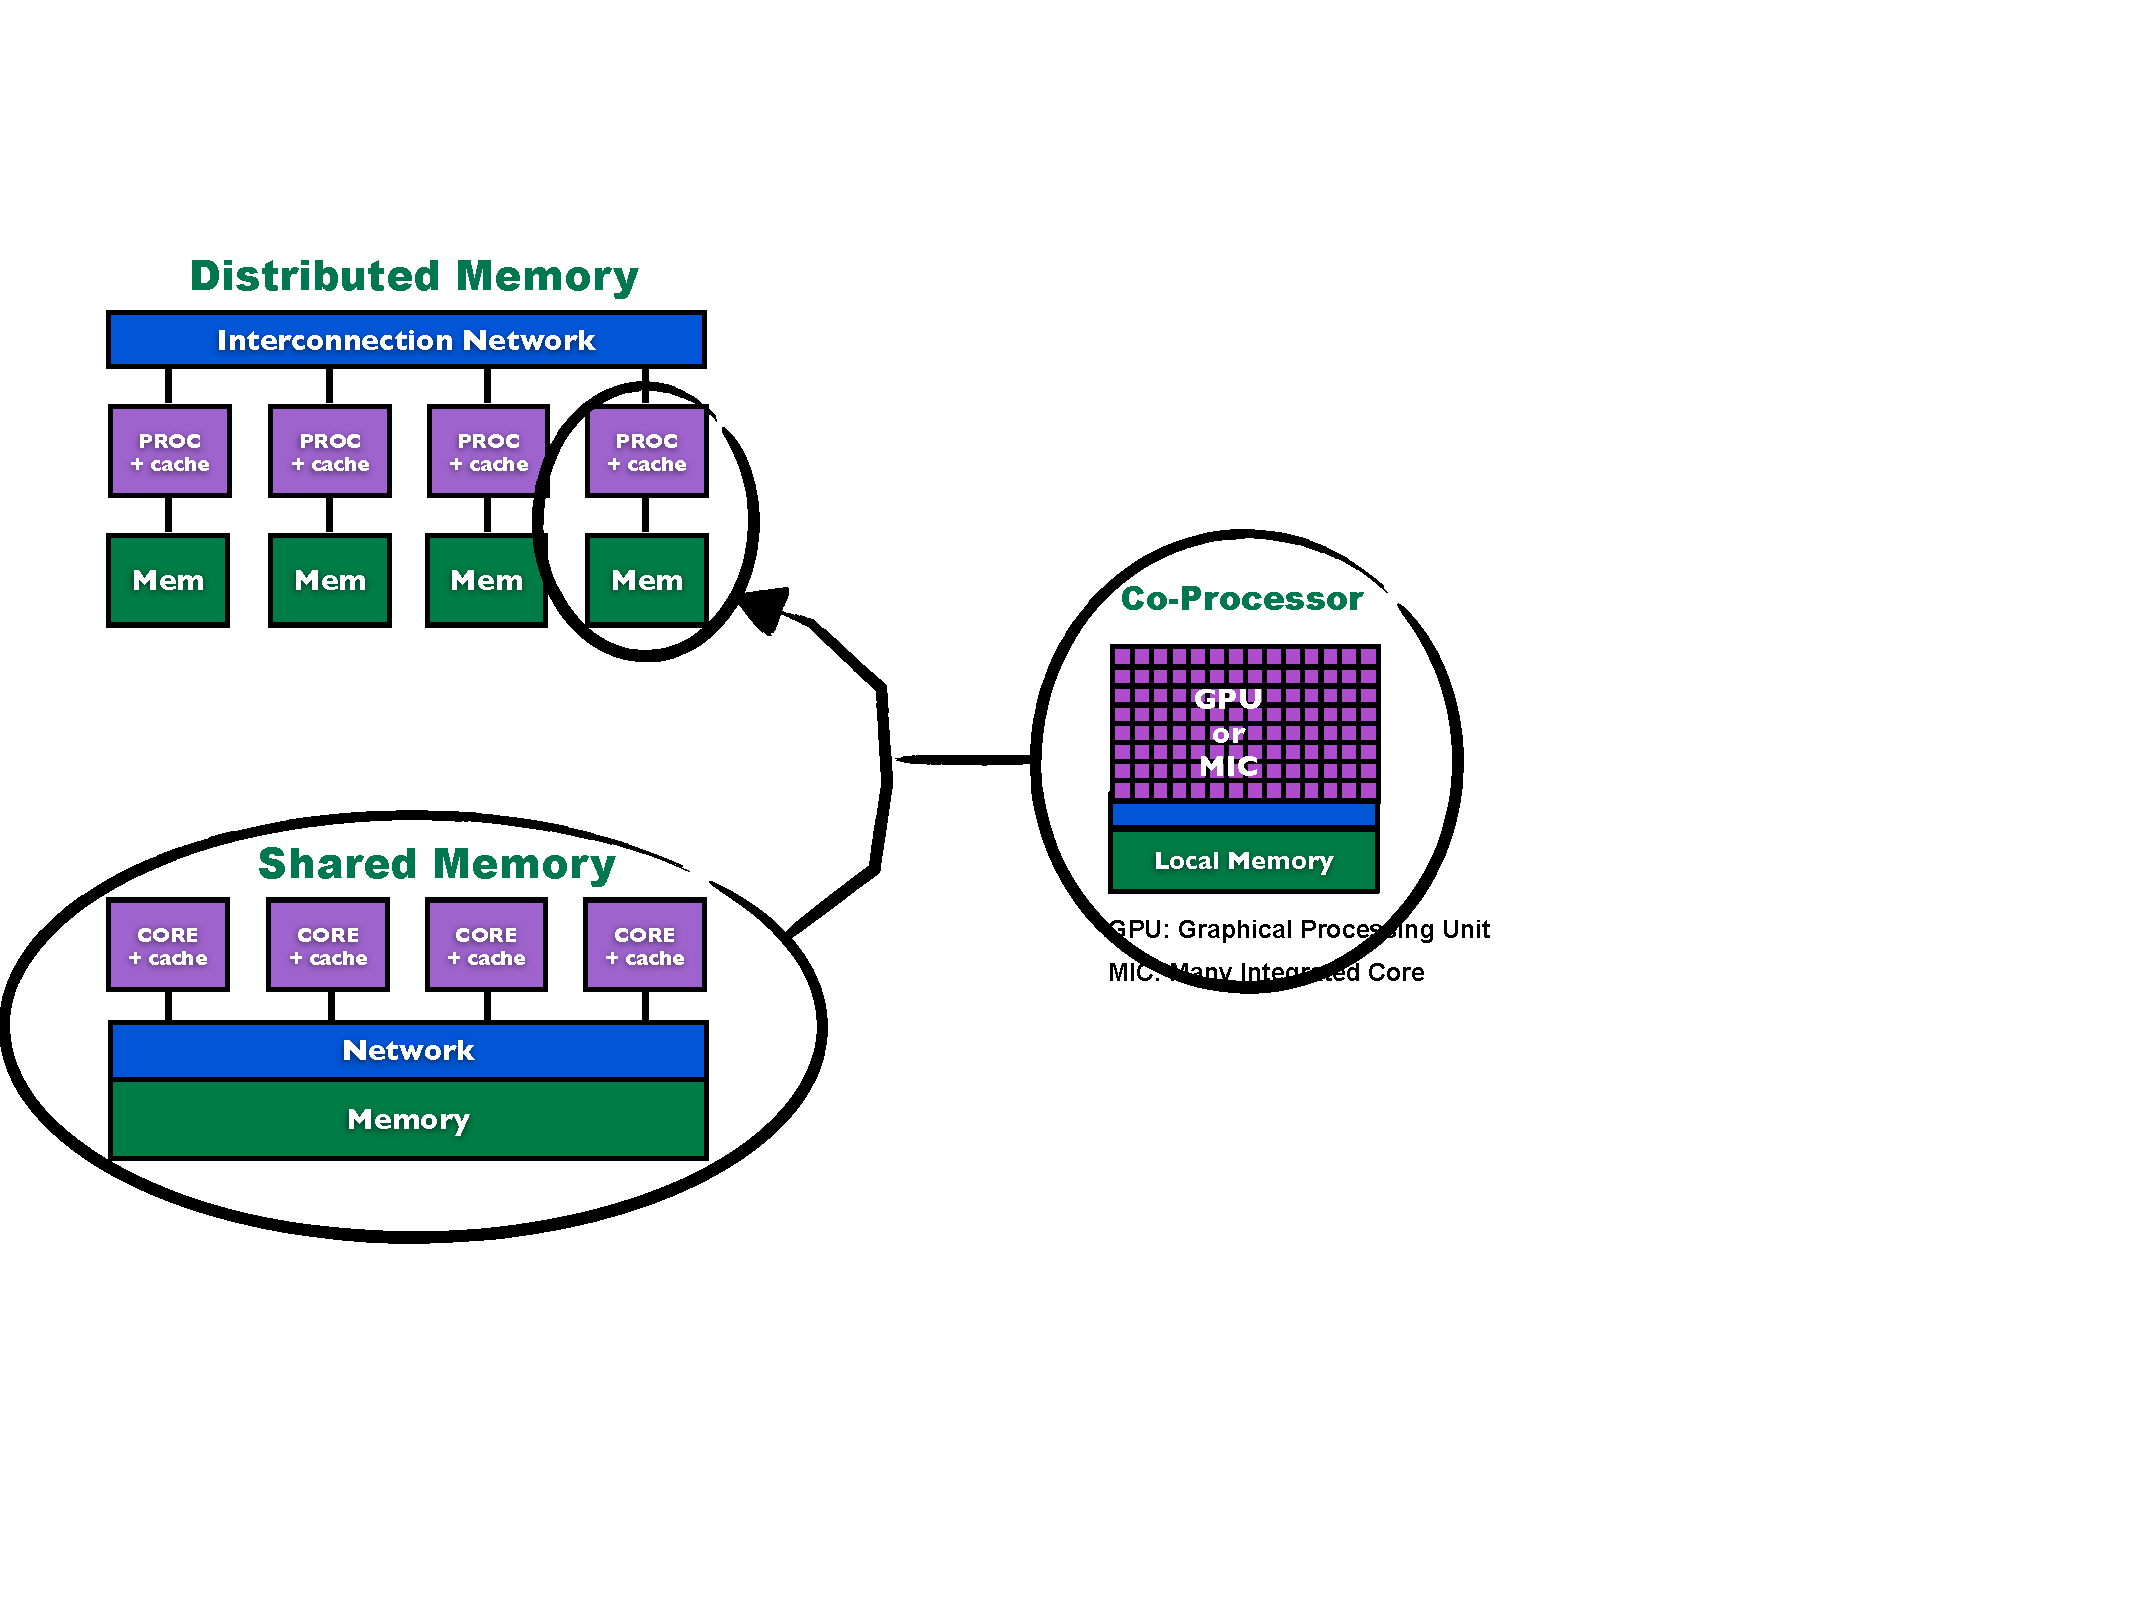
\includegraphics[width=0.95\textwidth]
{../common/pics/hardware/ParallelHardware4.pdf}
\end{frame}

\begin{frame}{Knowing the Right Words}
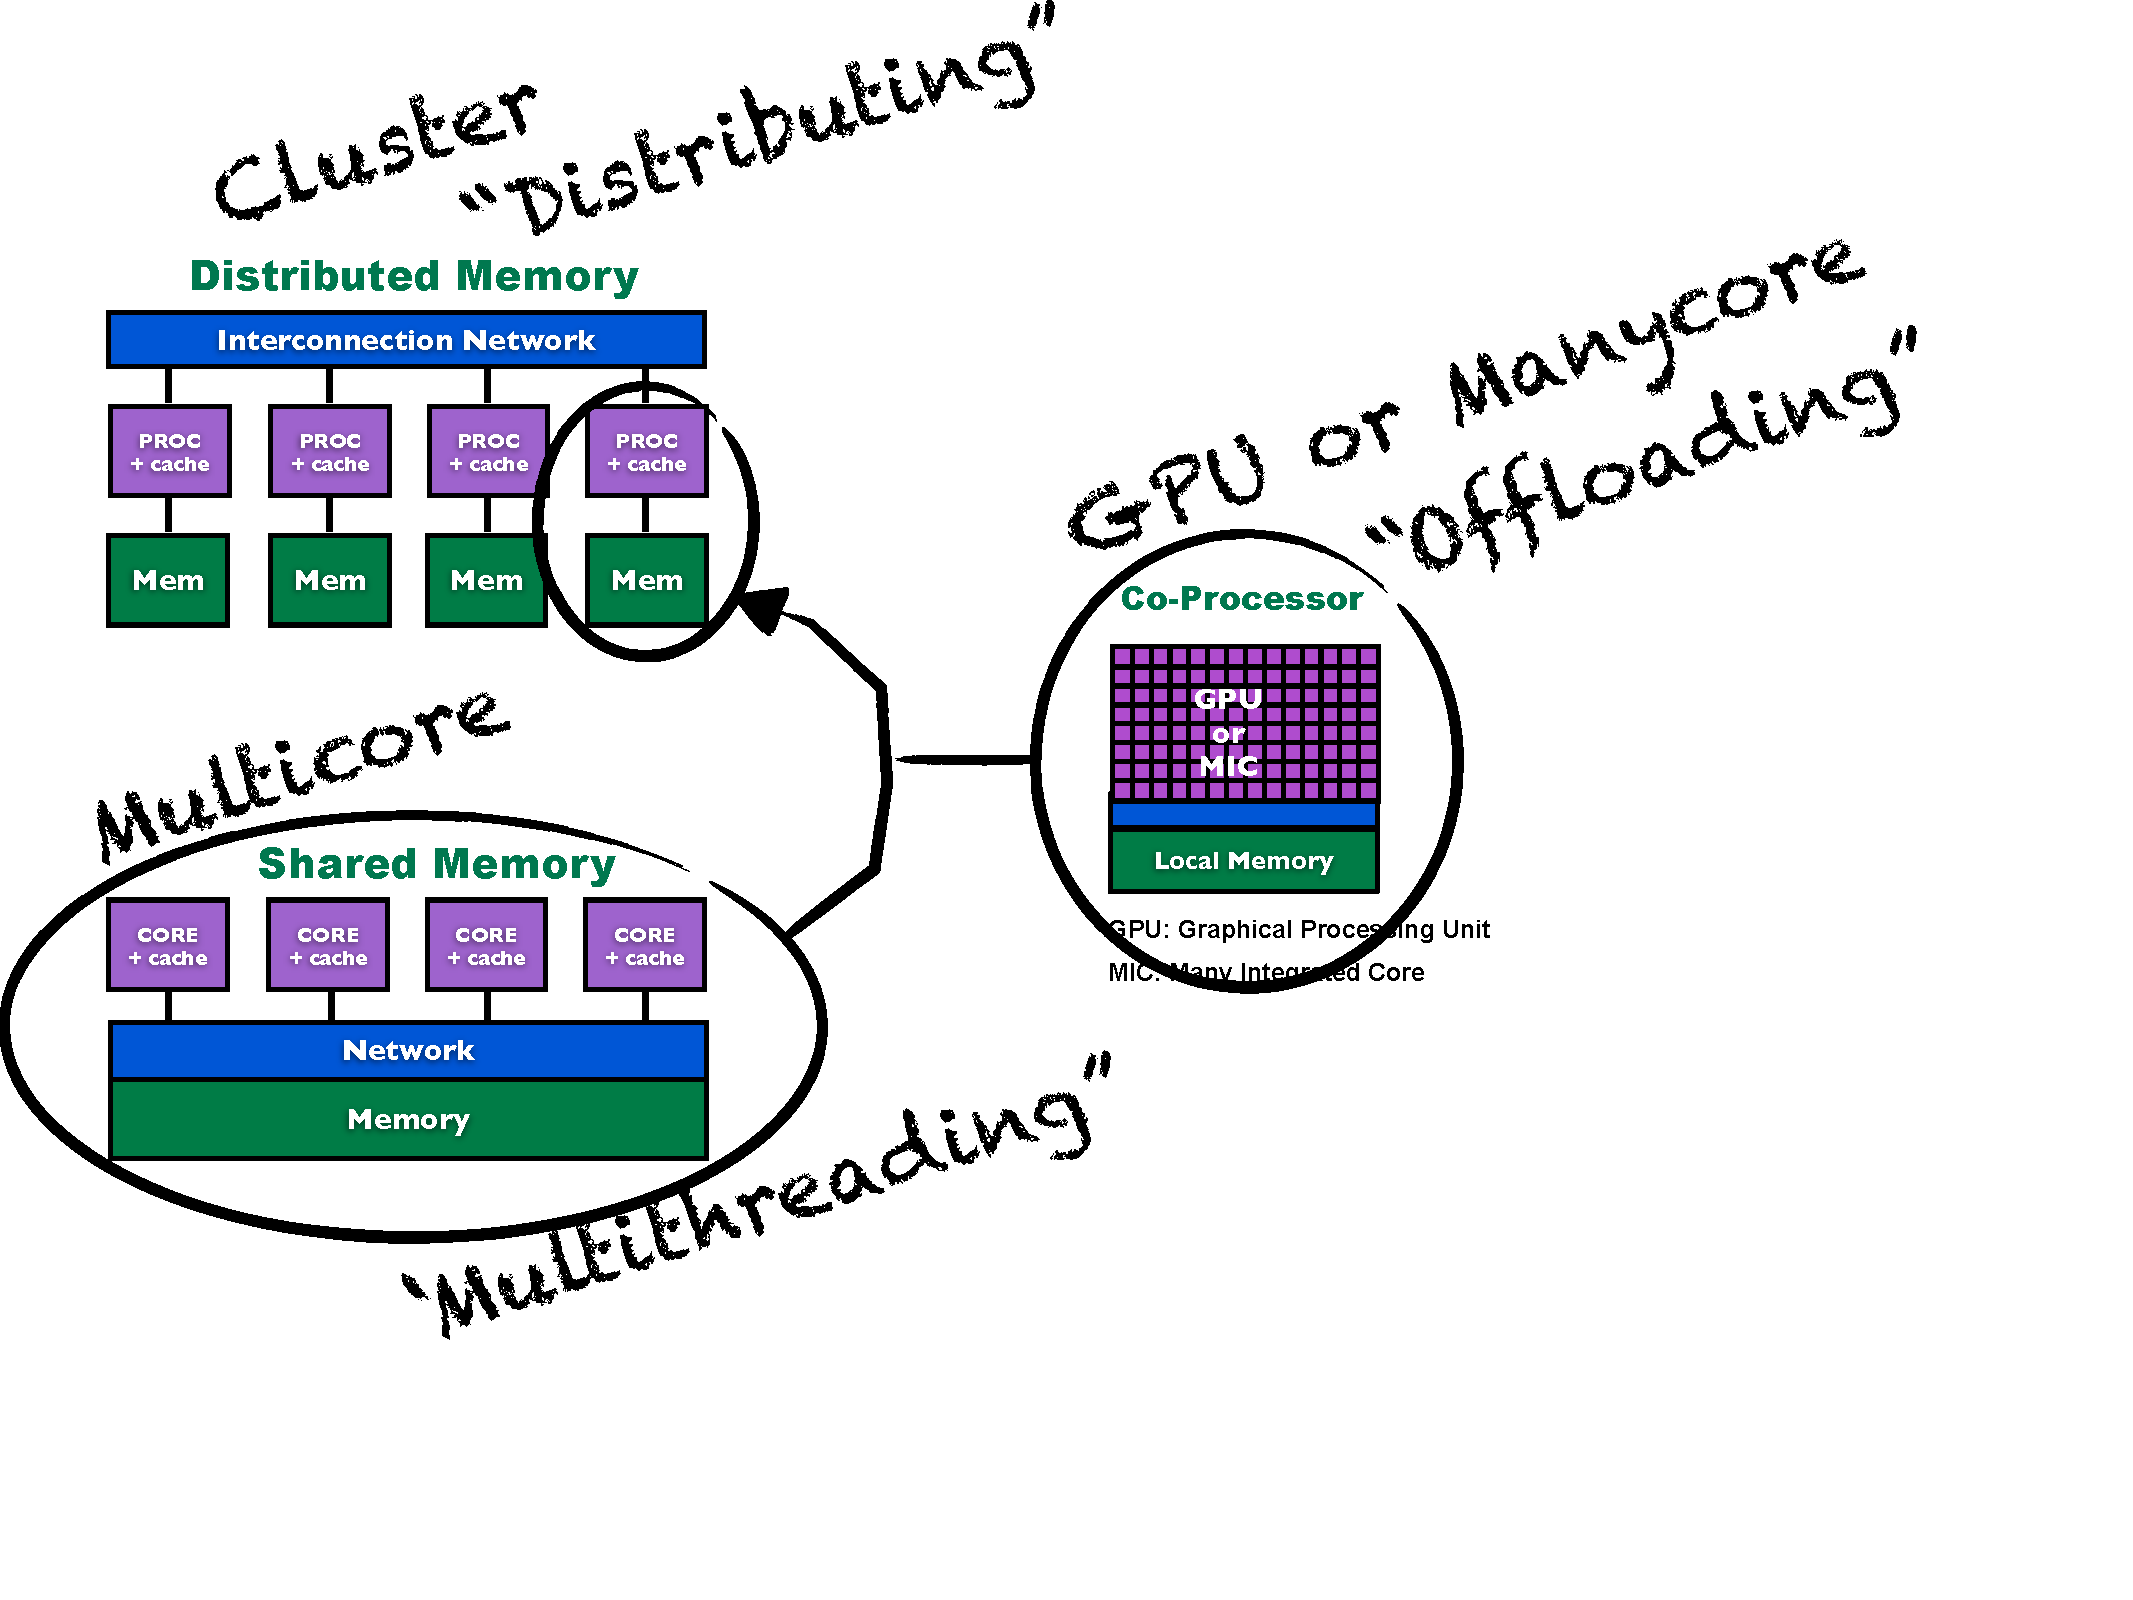
\includegraphics[width=0.95\textwidth]
{../common/pics/hardware/ParallelHardware5.pdf}
\end{frame}

\subsection{A Quick Overview of Parallel Software}
\makesubcontentsslidessec

\begin{frame}{``Native'' Programming Models and Tools}
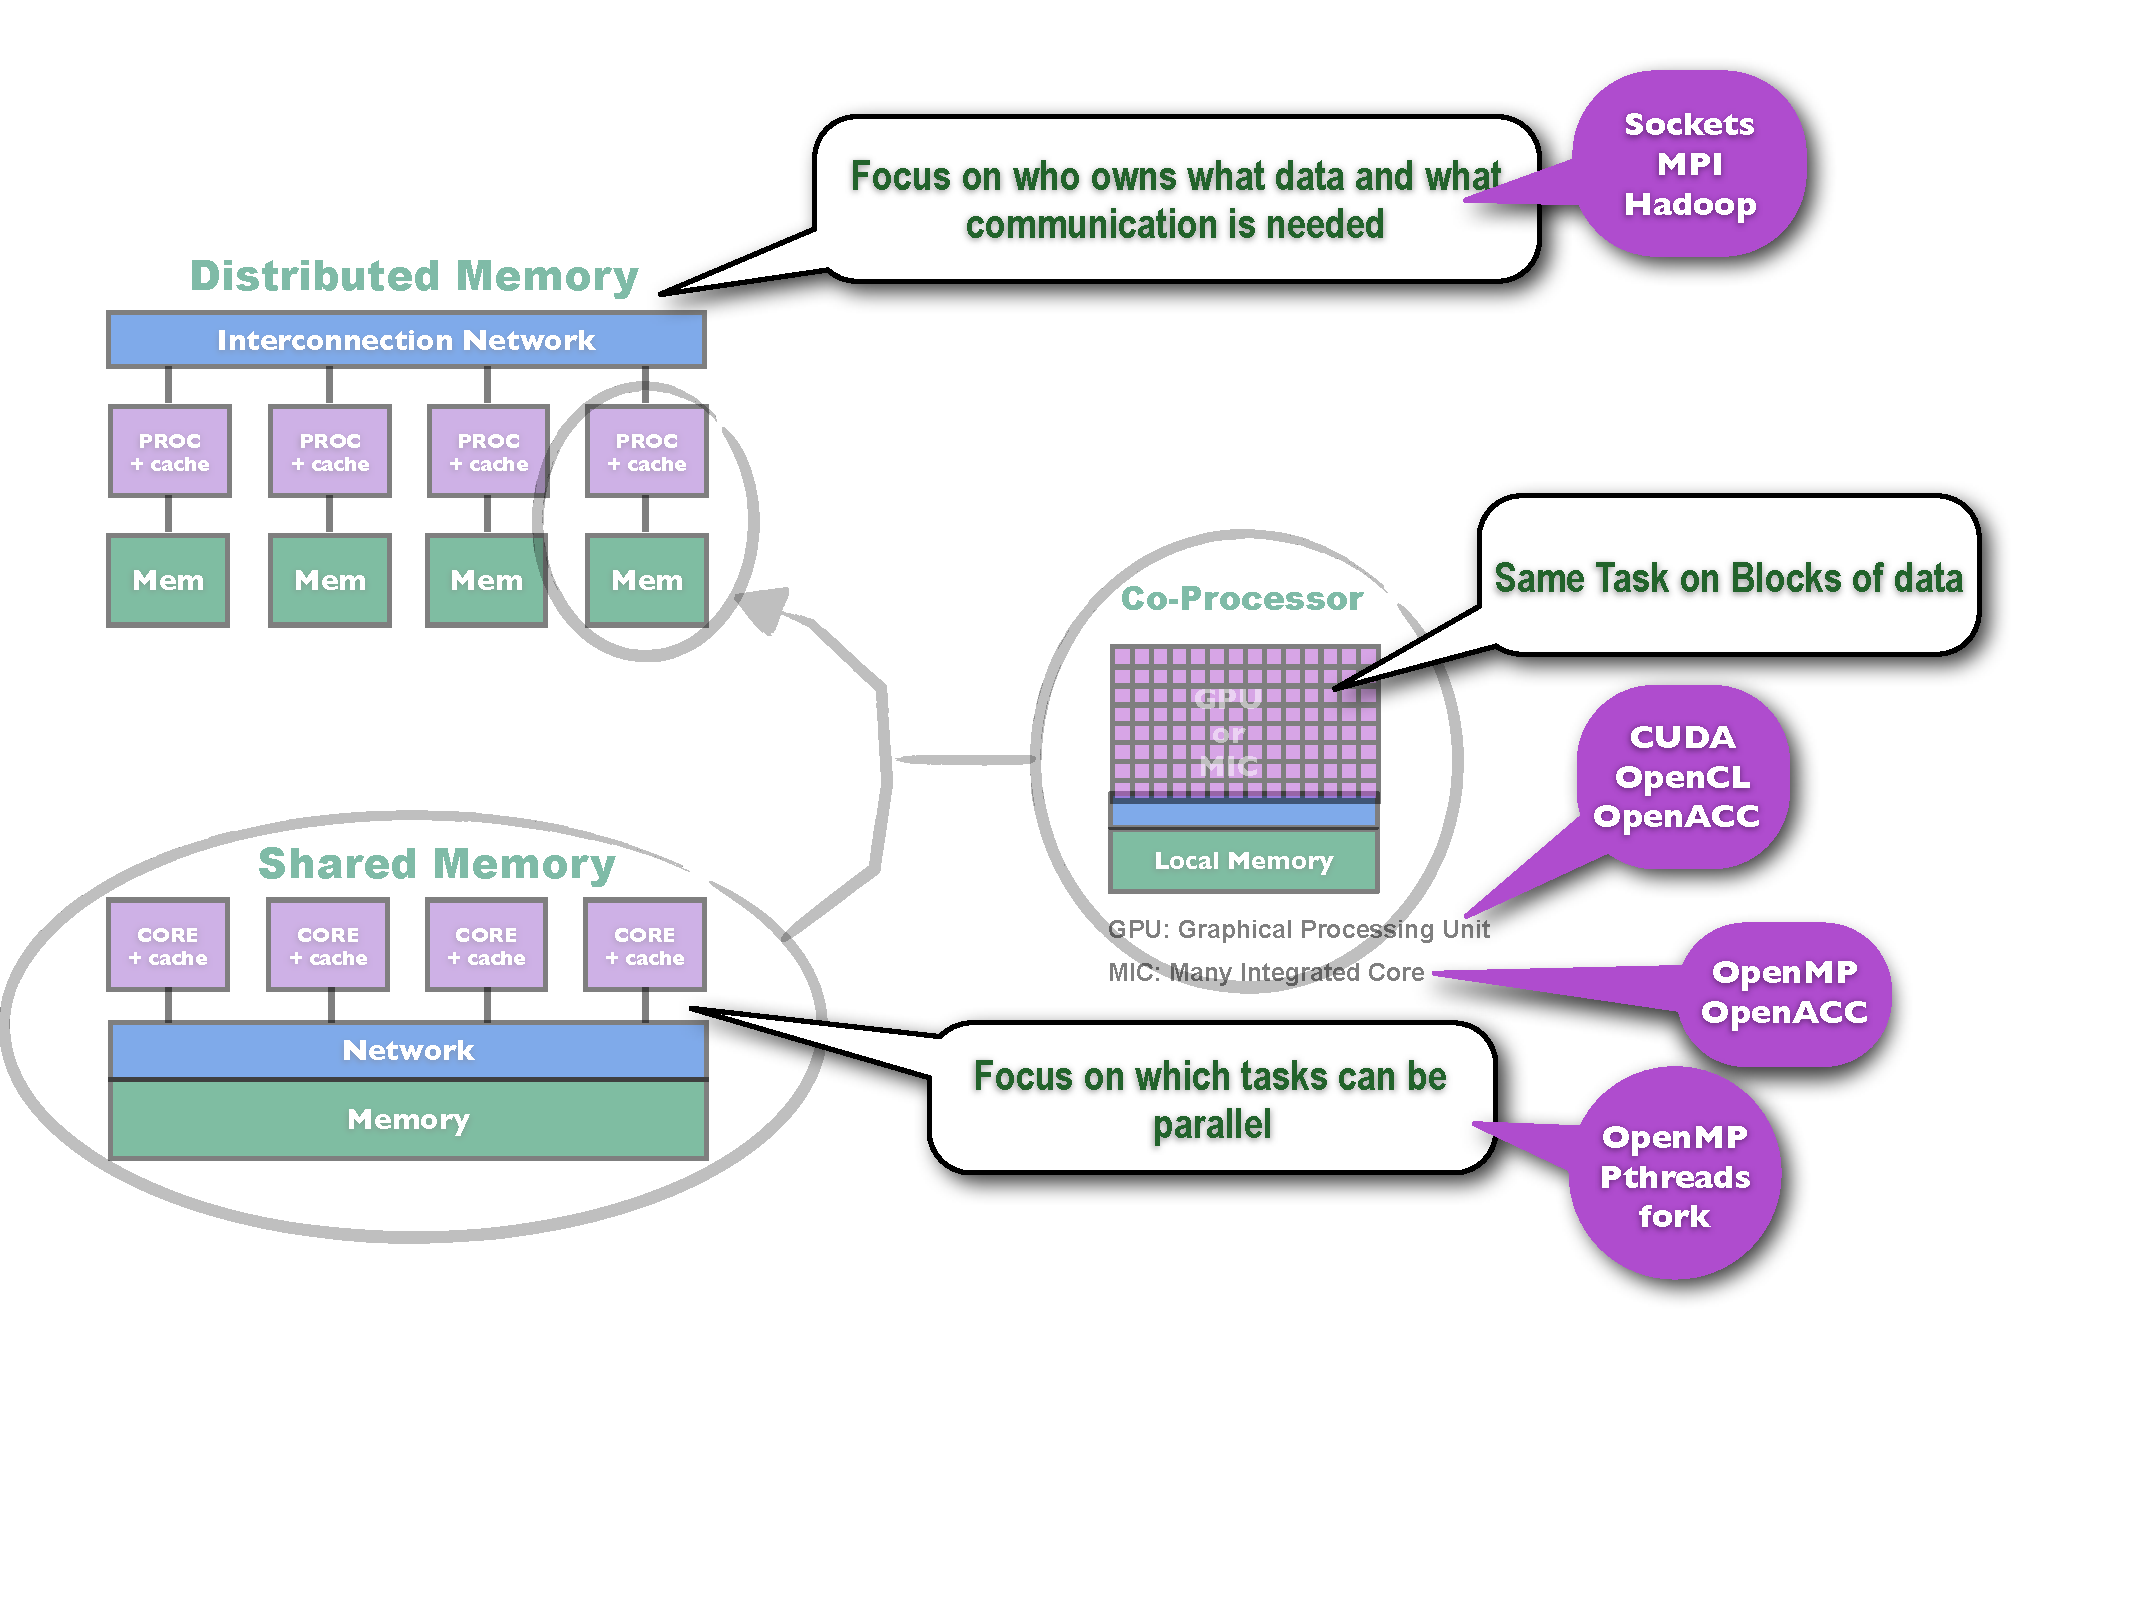
\includegraphics[width=0.95\textwidth]
{../common/pics/hardware/ParallelHardware6.pdf}
\end{frame}

\begin{frame}{30+ Years of Parallel Computing Research}
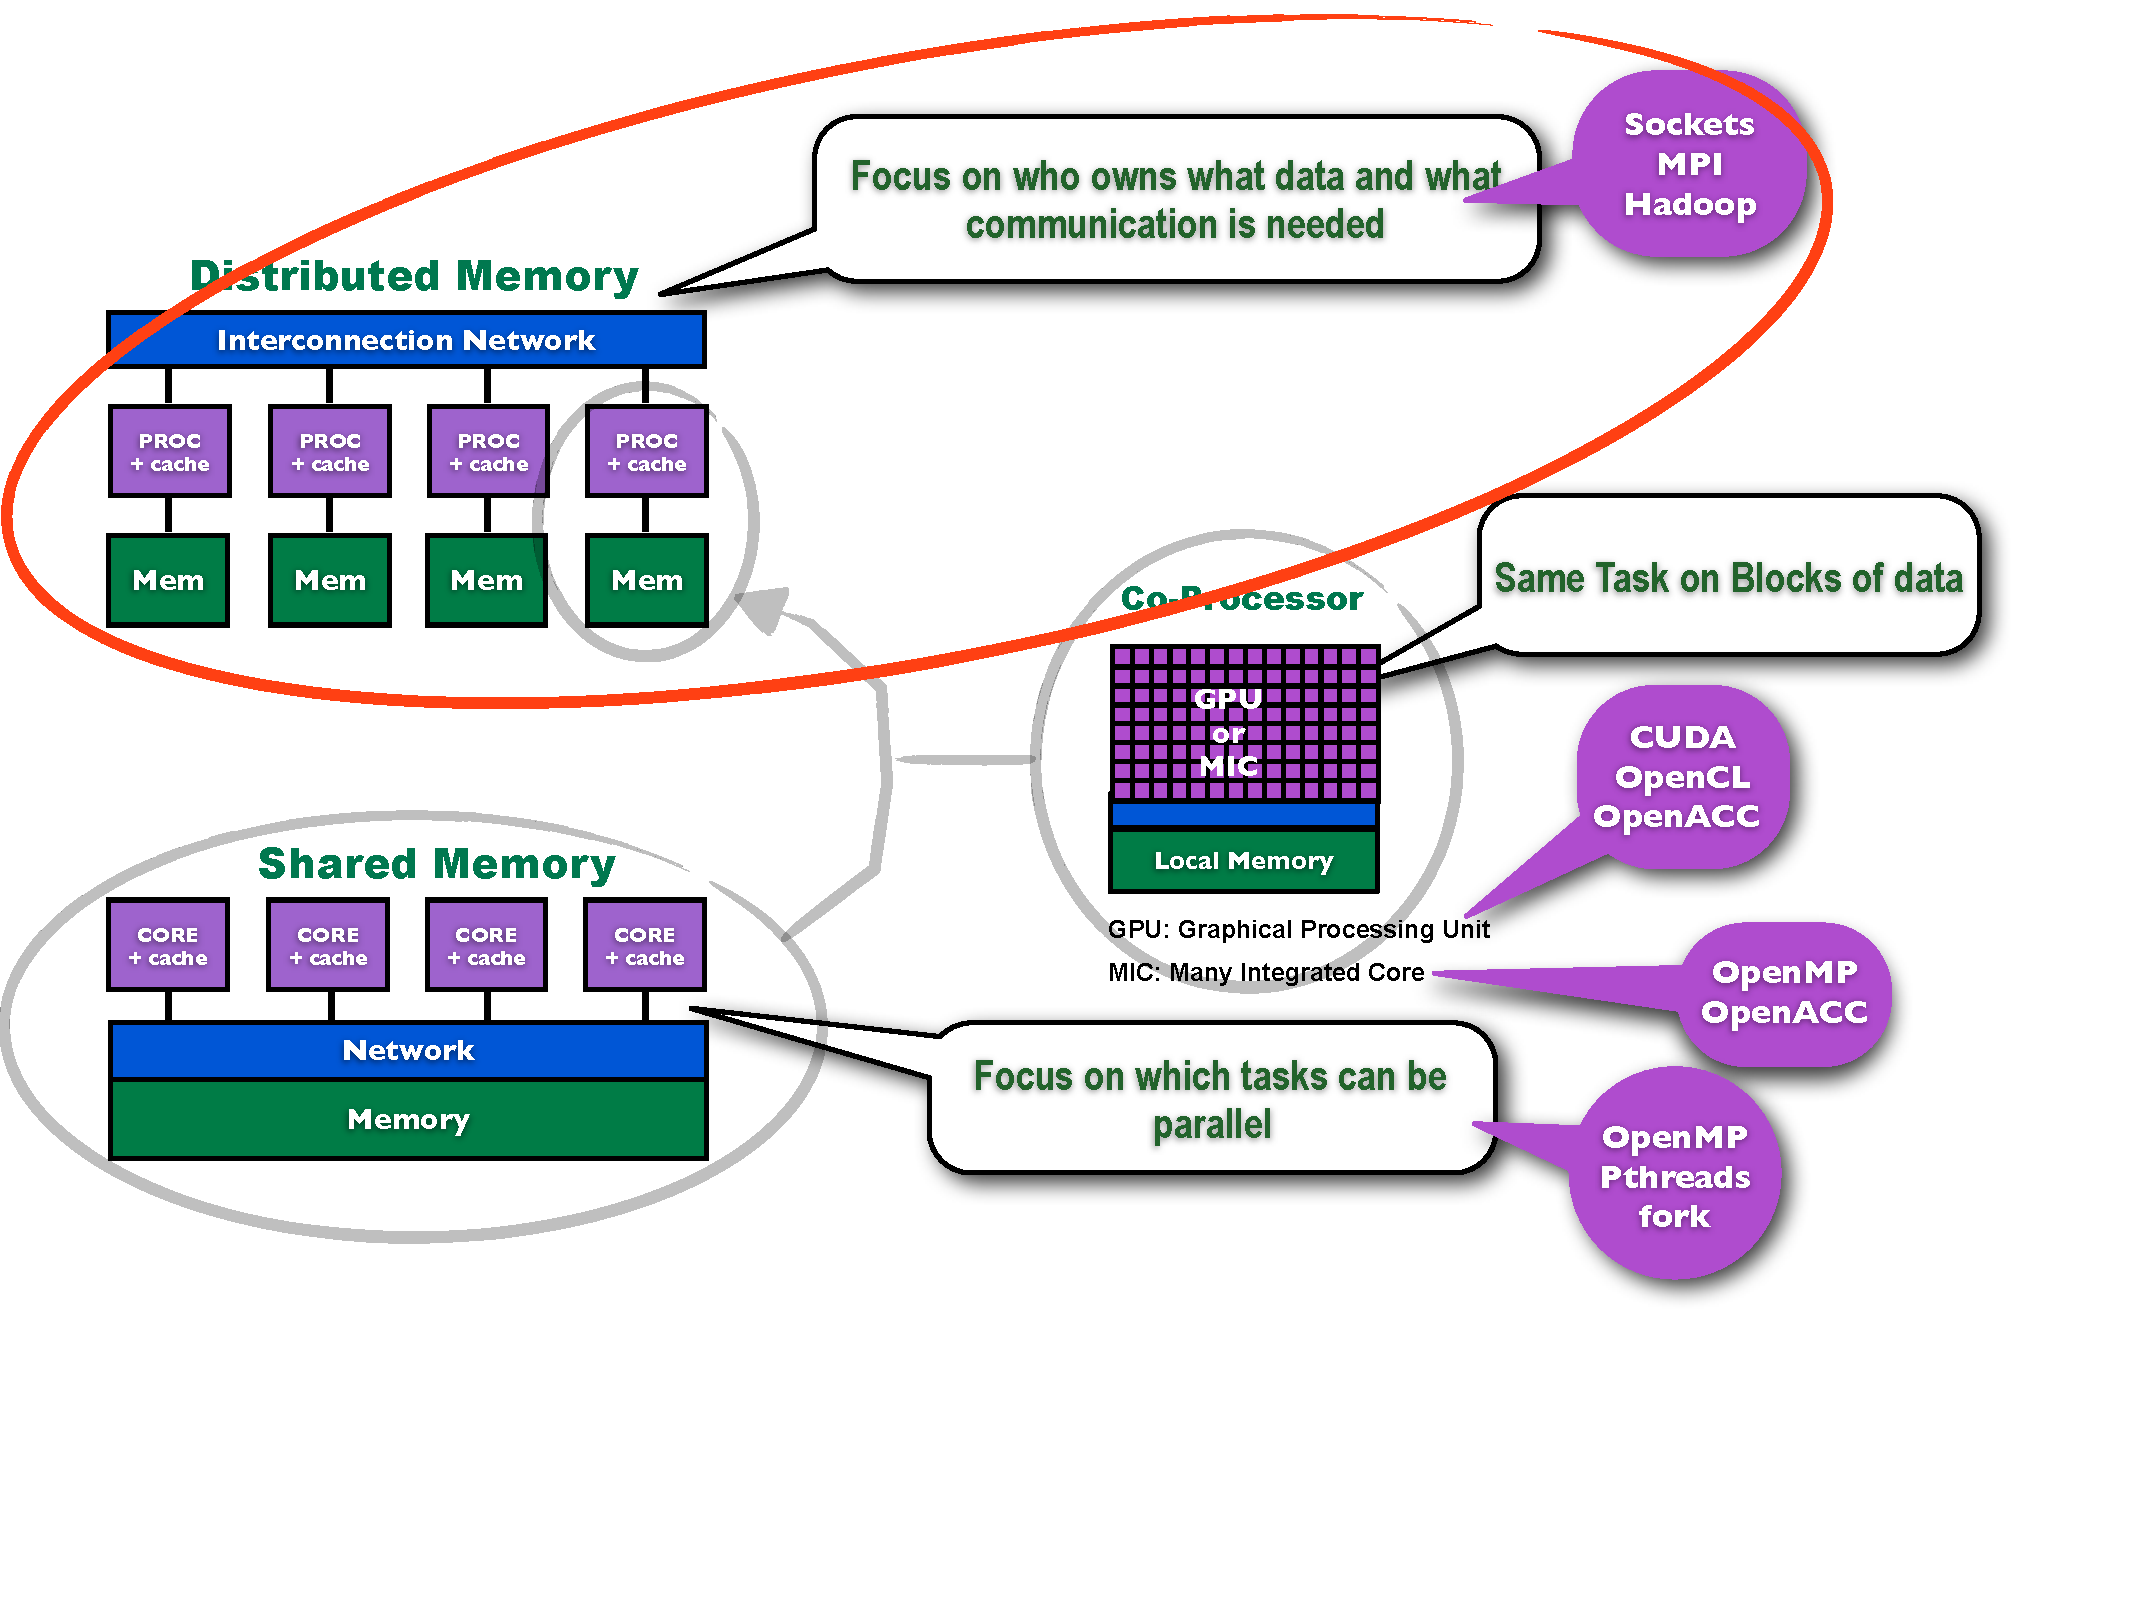
\includegraphics[width=0.95\textwidth]
{../common/pics/hardware/ParallelHardware7.pdf}
\end{frame}

\begin{frame}{Last 10 years of Advances}
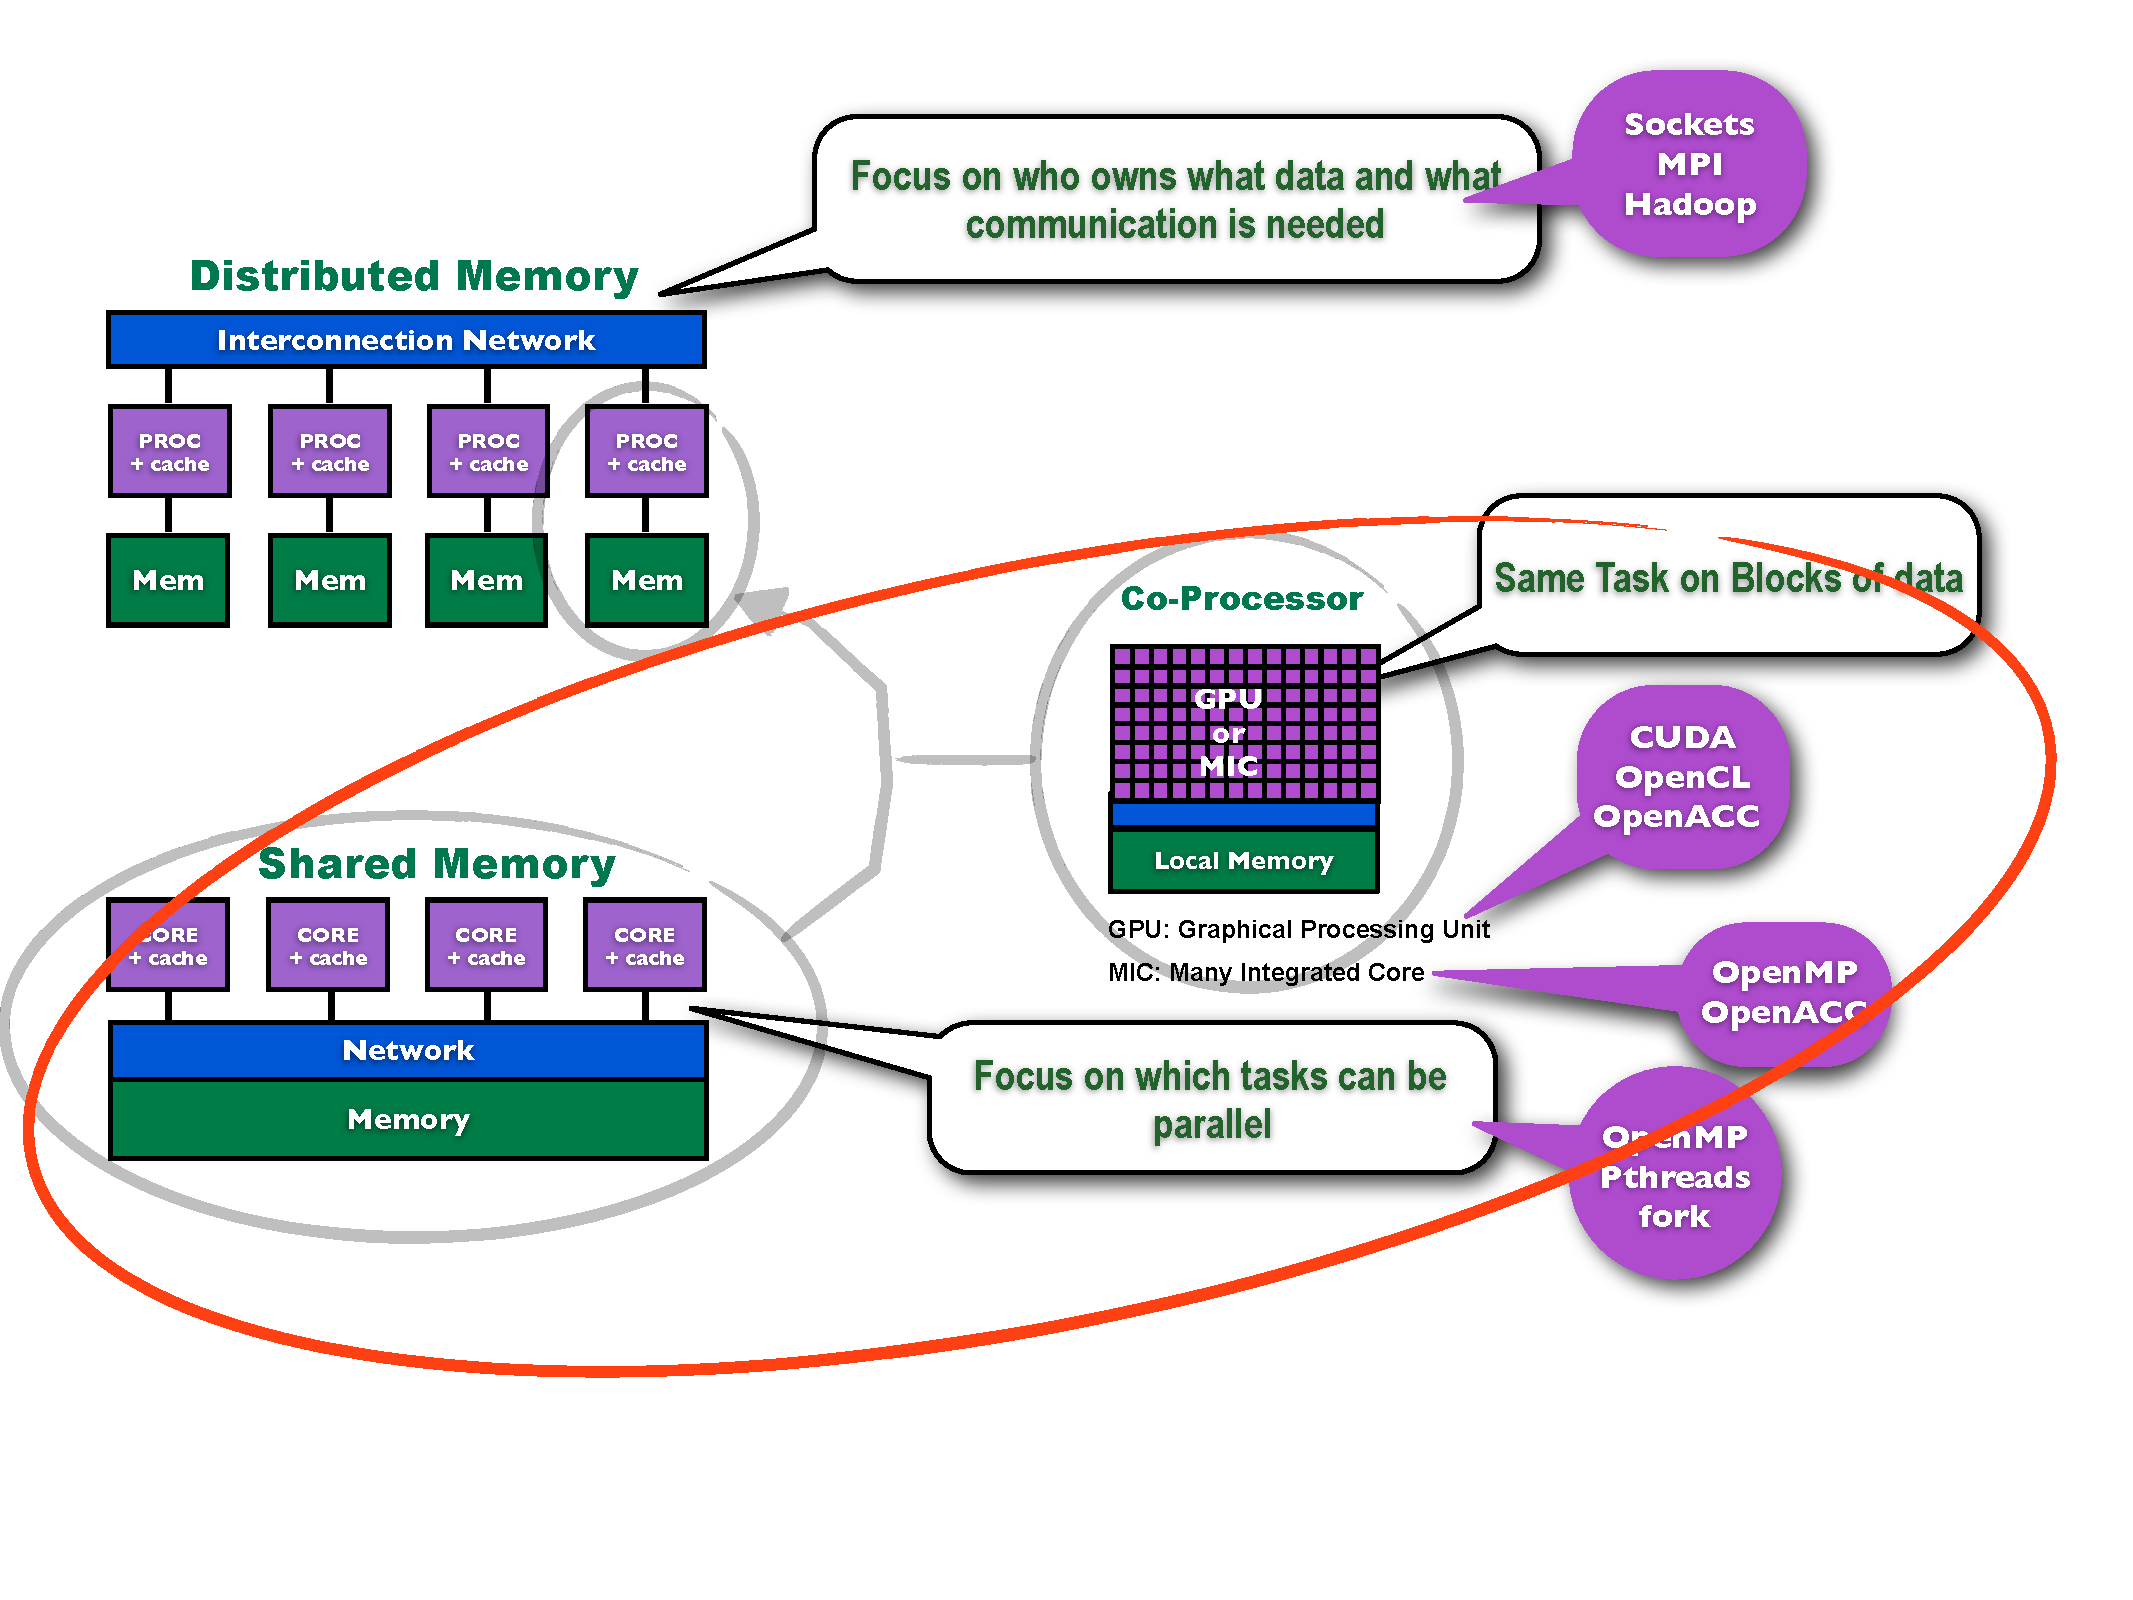
\includegraphics[width=0.95\textwidth]
{../common/pics/hardware/ParallelHardware8.pdf}
\end{frame}

\begin{frame}{Putting It All Together Challenge}
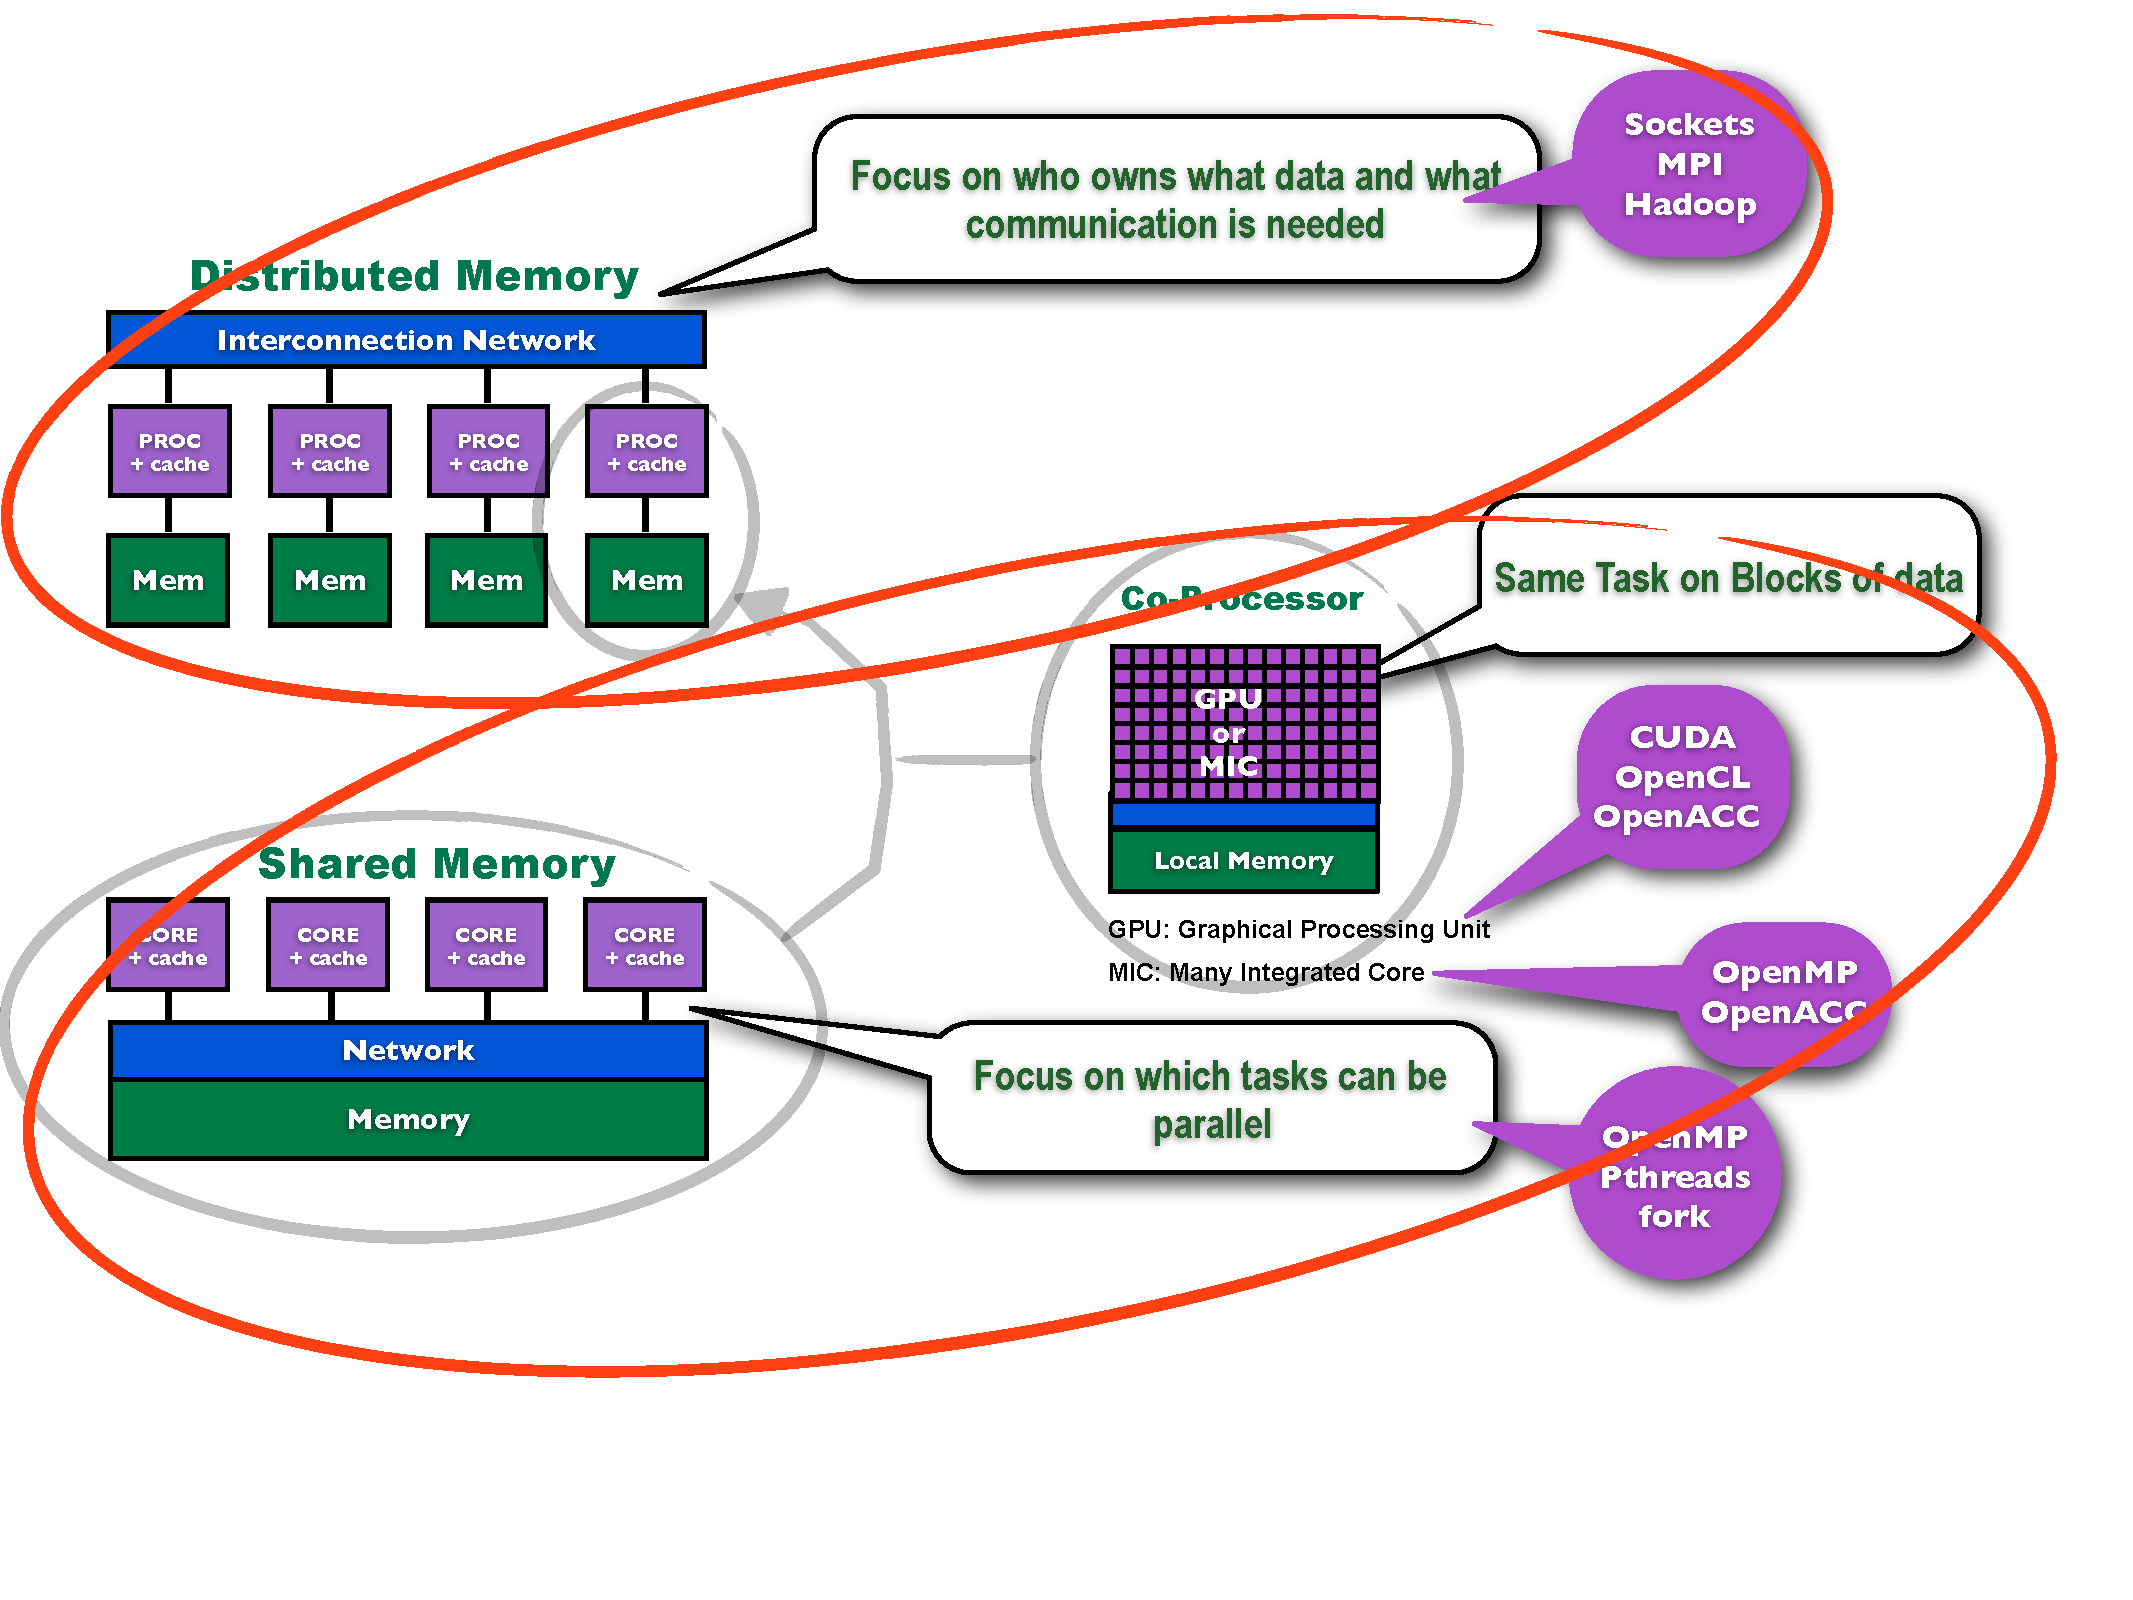
\includegraphics[width=0.95\textwidth]
{../common/pics/hardware/ParallelHardware9.pdf}
\end{frame}

\begin{frame}{R Interfaces to Native Tools}
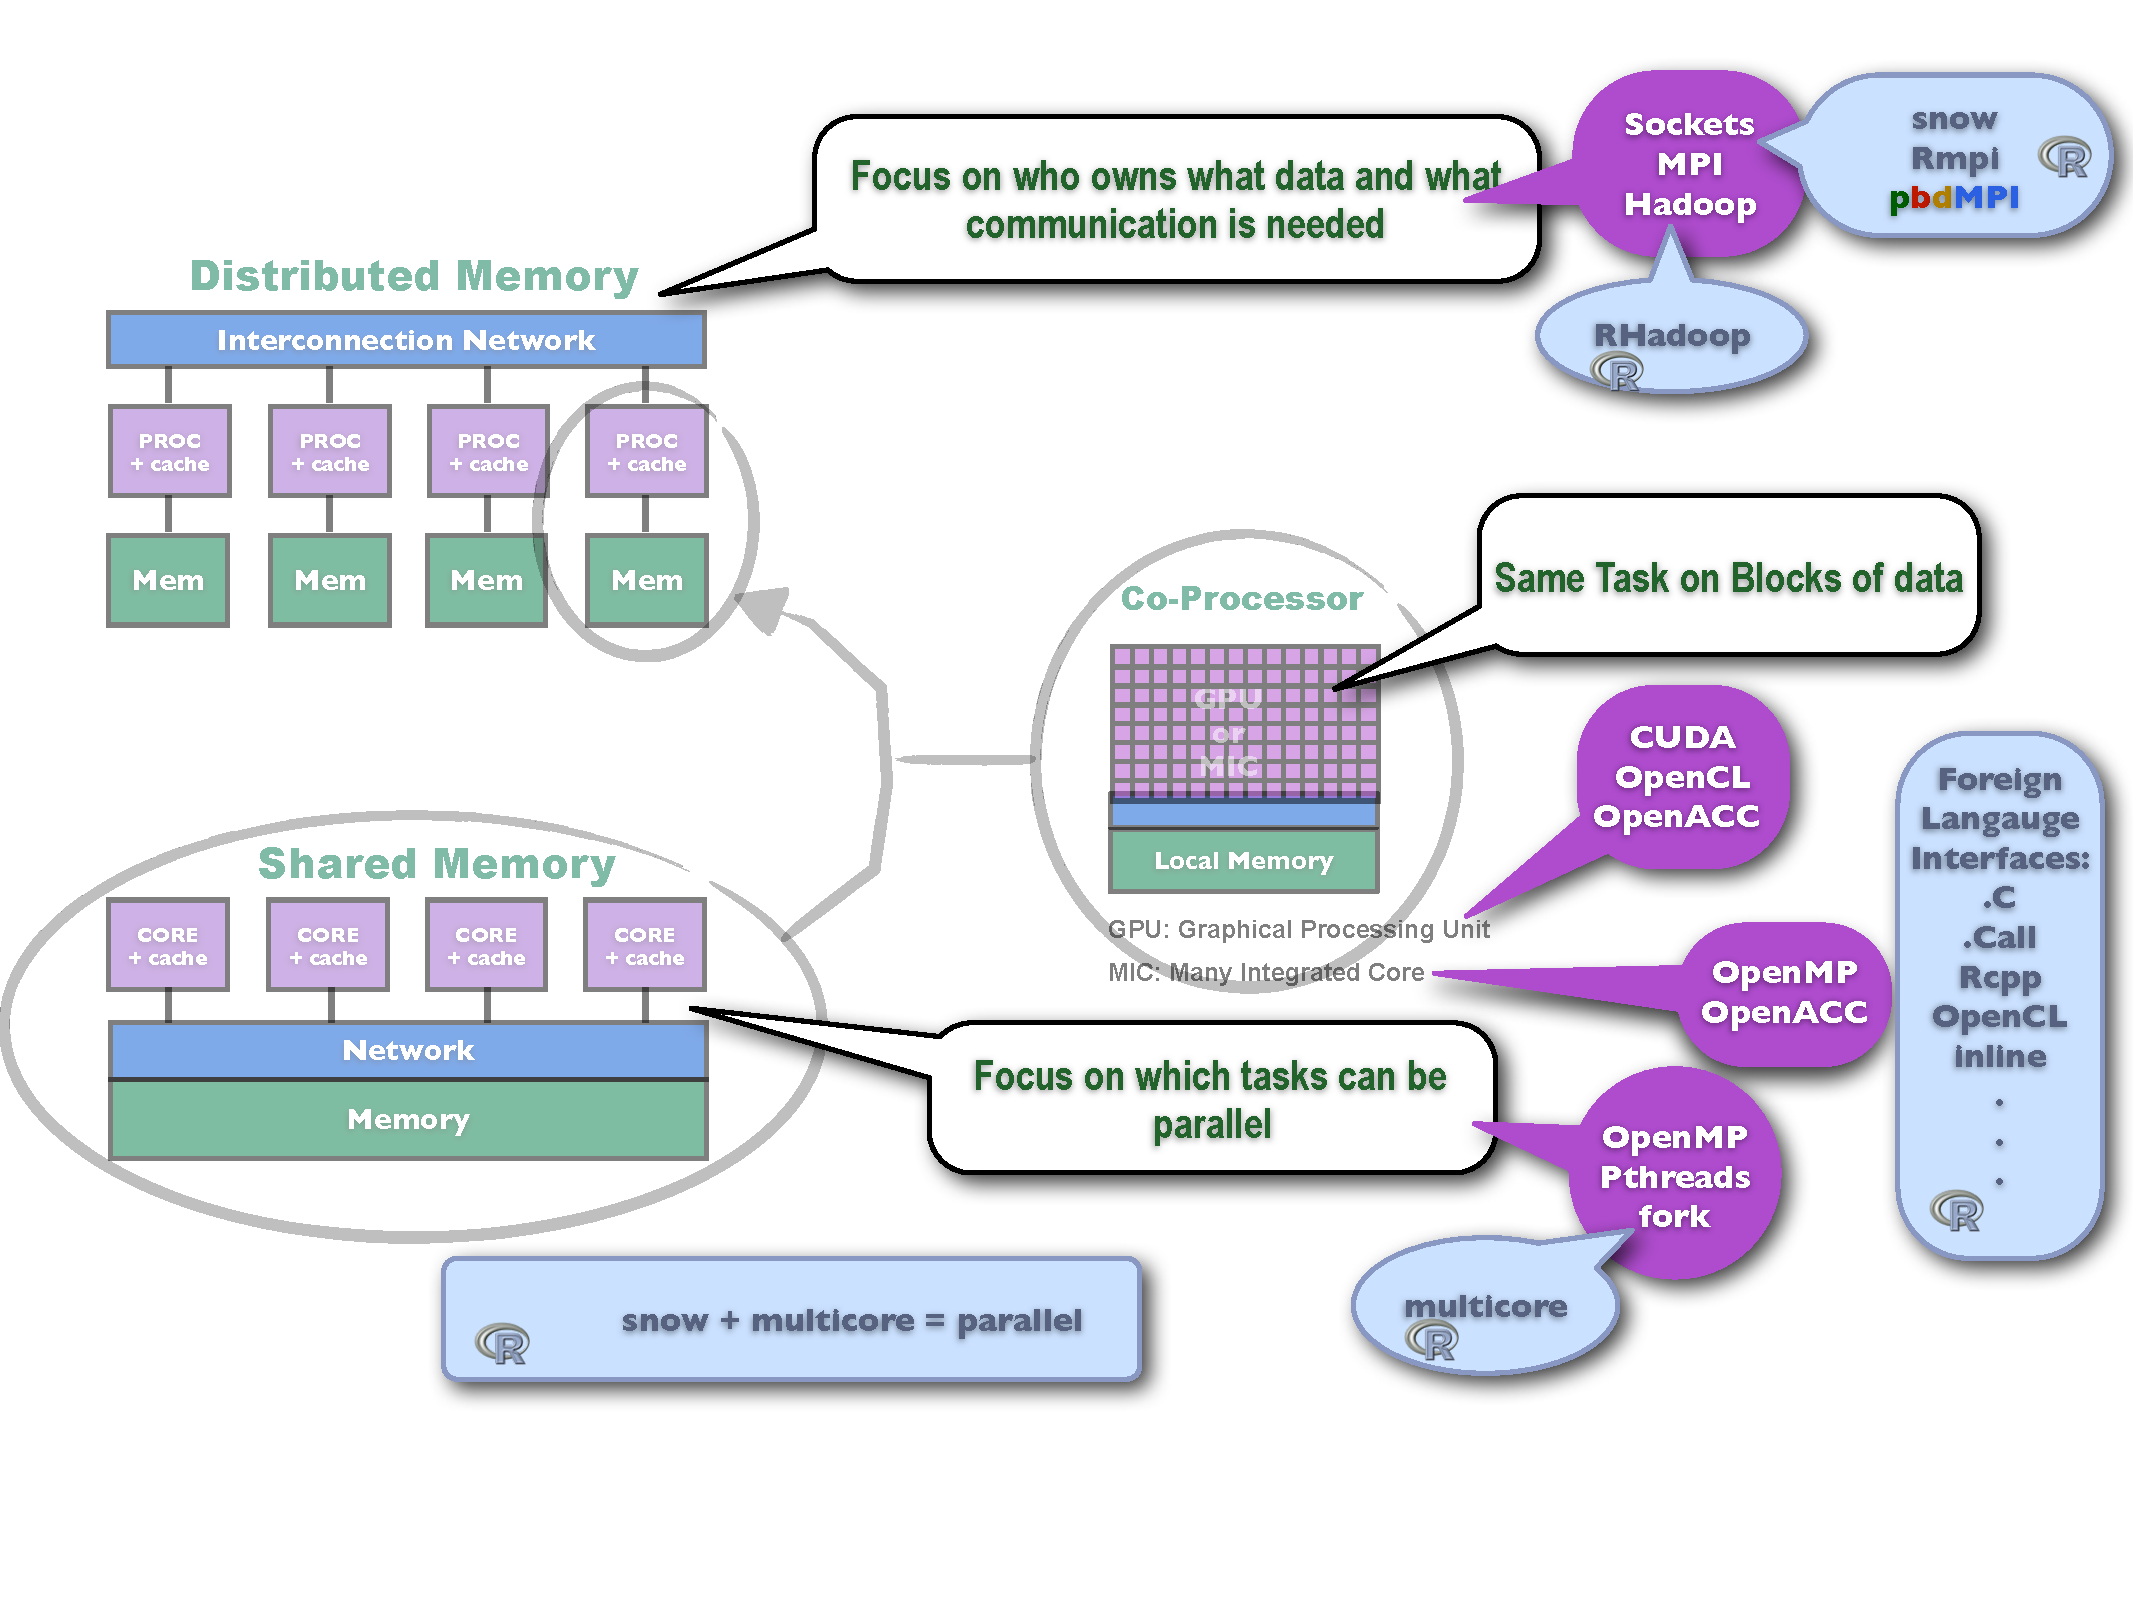
\includegraphics[width=0.95\textwidth]
{../common/pics/hardware/ParallelHardware10.pdf}
\end{frame}

